\documentclass[1p]{elsarticle_modified}
%\bibliographystyle{elsarticle-num}

%\usepackage[colorlinks]{hyperref}
%\usepackage{abbrmath_seonhwa} %\Abb, \Ascr, \Acal ,\Abf, \Afrak
\usepackage{amsfonts}
\usepackage{amssymb}
\usepackage{amsmath}
\usepackage{amsthm}
\usepackage{scalefnt}
\usepackage{amsbsy}
\usepackage{kotex}
\usepackage{caption}
\usepackage{subfig}
\usepackage{color}
\usepackage{graphicx}
\usepackage{xcolor} %% white, black, red, green, blue, cyan, magenta, yellow
\usepackage{float}
\usepackage{setspace}
\usepackage{hyperref}

\usepackage{tikz}
\usetikzlibrary{arrows}

\usepackage{multirow}
\usepackage{array} % fixed length table
\usepackage{hhline}

%%%%%%%%%%%%%%%%%%%%%
\makeatletter
\renewcommand*\env@matrix[1][\arraystretch]{%
	\edef\arraystretch{#1}%
	\hskip -\arraycolsep
	\let\@ifnextchar\new@ifnextchar
	\array{*\c@MaxMatrixCols c}}
\makeatother %https://tex.stackexchange.com/questions/14071/how-can-i-increase-the-line-spacing-in-a-matrix
%%%%%%%%%%%%%%%

\usepackage[normalem]{ulem}

\newcommand{\msout}[1]{\ifmmode\text{\sout{\ensuremath{#1}}}\else\sout{#1}\fi}
%SOURCE: \msout is \stkout macro in https://tex.stackexchange.com/questions/20609/strikeout-in-math-mode

\newcommand{\cancel}[1]{
	\ifmmode
	{\color{red}\msout{#1}}
	\else
	{\color{red}\sout{#1}}
	\fi
}

\newcommand{\add}[1]{
	{\color{blue}\uwave{#1}}
}

\newcommand{\replace}[2]{
	\ifmmode
	{\color{red}\msout{#1}}{\color{blue}\uwave{#2}}
	\else
	{\color{red}\sout{#1}}{\color{blue}\uwave{#2}}
	\fi
}

\newcommand{\Sol}{\mathcal{S}} %segment
\newcommand{\D}{D} %diagram
\newcommand{\A}{\mathcal{A}} %arc


%%%%%%%%%%%%%%%%%%%%%%%%%%%%%5 test

\def\sl{\operatorname{\textup{SL}}(2,\Cbb)}
\def\psl{\operatorname{\textup{PSL}}(2,\Cbb)}
\def\quan{\mkern 1mu \triangleright \mkern 1mu}

\theoremstyle{definition}
\newtheorem{thm}{Theorem}[section]
\newtheorem{prop}[thm]{Proposition}
\newtheorem{lem}[thm]{Lemma}
\newtheorem{ques}[thm]{Question}
\newtheorem{cor}[thm]{Corollary}
\newtheorem{defn}[thm]{Definition}
\newtheorem{exam}[thm]{Example}
\newtheorem{rmk}[thm]{Remark}
\newtheorem{alg}[thm]{Algorithm}

\newcommand{\I}{\sqrt{-1}}
\begin{document}

%\begin{frontmatter}
%
%\title{Boundary parabolic representations of knots up to 8 crossings}
%
%%% Group authors per affiliation:
%\author{Yunhi Cho} 
%\address{Department of Mathematics, University of Seoul, Seoul, Korea}
%\ead{yhcho@uos.ac.kr}
%
%
%\author{Seonhwa Kim} %\fnref{s_kim}}
%\address{Center for Geometry and Physics, Institute for Basic Science, Pohang, 37673, Korea}
%\ead{ryeona17@ibs.re.kr}
%
%\author{Hyuk Kim}
%\address{Department of Mathematical Sciences, Seoul National University, Seoul 08826, Korea}
%\ead{hyukkim@snu.ac.kr}
%
%\author{Seokbeom Yoon}
%\address{Department of Mathematical Sciences, Seoul National University, Seoul, 08826,  Korea}
%\ead{sbyoon15@snu.ac.kr}
%
%\begin{abstract}
%We find all boundary parabolic representation of knots up to 8 crossings.
%
%\end{abstract}
%\begin{keyword}
%    \MSC[2010] 57M25 
%\end{keyword}
%
%\end{frontmatter}

%\linenumbers
%\tableofcontents
%
\newcommand\colored[1]{\textcolor{white}{\rule[-0.35ex]{0.8em}{1.4ex}}\kern-0.8em\color{red} #1}%
%\newcommand\colored[1]{\textcolor{white}{ #1}\kern-2.17ex	\textcolor{white}{ #1}\kern-1.81ex	\textcolor{white}{ #1}\kern-2.15ex\color{red}#1	}

{\Large $\underline{12n_{0884}~(K12n_{0884})}$}

\setlength{\tabcolsep}{10pt}
\renewcommand{\arraystretch}{1.6}
\vspace{1cm}\begin{tabular}{m{100pt}>{\centering\arraybackslash}m{274pt}}
\multirow{5}{120pt}{
	\centering
	\includegraphics[width=112pt]{../../../GIT/diagram.site/Diagrams/png/2973_12n_0884.png}\\
\ \ \ A knot diagram\footnotemark}&
\allowdisplaybreaks
\textbf{Linearized knot diagam} \\
\cline{2-2}
 &
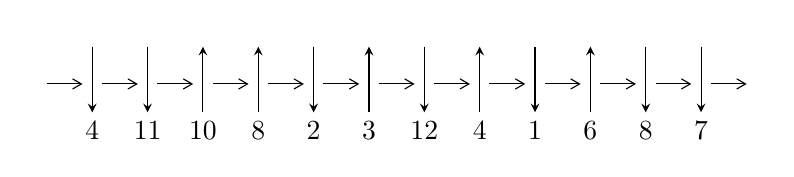
\begin{tikzpicture}[x=20pt, y=17pt]
	% nodes
	\node (C0) at (0, 0) {};
	\node (C1) at (1, 0) {};
	\node (C1U) at (1, +1) {};
	\node (C1D) at (1, -1) {4};

	\node (C2) at (2, 0) {};
	\node (C2U) at (2, +1) {};
	\node (C2D) at (2, -1) {11};

	\node (C3) at (3, 0) {};
	\node (C3U) at (3, +1) {};
	\node (C3D) at (3, -1) {10};

	\node (C4) at (4, 0) {};
	\node (C4U) at (4, +1) {};
	\node (C4D) at (4, -1) {8};

	\node (C5) at (5, 0) {};
	\node (C5U) at (5, +1) {};
	\node (C5D) at (5, -1) {2};

	\node (C6) at (6, 0) {};
	\node (C6U) at (6, +1) {};
	\node (C6D) at (6, -1) {3};

	\node (C7) at (7, 0) {};
	\node (C7U) at (7, +1) {};
	\node (C7D) at (7, -1) {12};

	\node (C8) at (8, 0) {};
	\node (C8U) at (8, +1) {};
	\node (C8D) at (8, -1) {4};

	\node (C9) at (9, 0) {};
	\node (C9U) at (9, +1) {};
	\node (C9D) at (9, -1) {1};

	\node (C10) at (10, 0) {};
	\node (C10U) at (10, +1) {};
	\node (C10D) at (10, -1) {6};

	\node (C11) at (11, 0) {};
	\node (C11U) at (11, +1) {};
	\node (C11D) at (11, -1) {8};

	\node (C12) at (12, 0) {};
	\node (C12U) at (12, +1) {};
	\node (C12D) at (12, -1) {7};
	\node (C13) at (13, 0) {};

	% arrows
	\draw[->,>={angle 60}]
	(C0) edge (C1) (C1) edge (C2) (C2) edge (C3) (C3) edge (C4) (C4) edge (C5) (C5) edge (C6) (C6) edge (C7) (C7) edge (C8) (C8) edge (C9) (C9) edge (C10) (C10) edge (C11) (C11) edge (C12) (C12) edge (C13) ;	\draw[->,>=stealth]
	(C1U) edge (C1D) (C2U) edge (C2D) (C3D) edge (C3U) (C4D) edge (C4U) (C5U) edge (C5D) (C6D) edge (C6U) (C7U) edge (C7D) (C8D) edge (C8U) (C9U) edge (C9D) (C10D) edge (C10U) (C11U) edge (C11D) (C12U) edge (C12D) ;
	\end{tikzpicture} \\
\hhline{~~} \\& 
\textbf{Solving Sequence} \\ \cline{2-2} 
 &
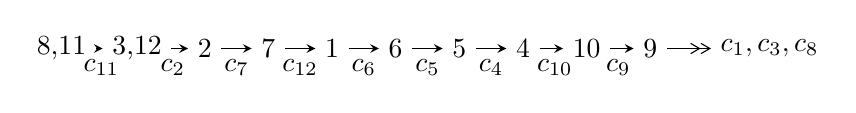
\begin{tikzpicture}[x=23pt, y=7pt]
	% node
	\node (A0) at (-1/8, 0) {8,11};
	\node (A1) at (17/16, 0) {3,12};
	\node (A2) at (17/8, 0) {2};
	\node (A3) at (25/8, 0) {7};
	\node (A4) at (33/8, 0) {1};
	\node (A5) at (41/8, 0) {6};
	\node (A6) at (49/8, 0) {5};
	\node (A7) at (57/8, 0) {4};
	\node (A8) at (65/8, 0) {10};
	\node (A9) at (73/8, 0) {9};
	\node (C1) at (1/2, -1) {$c_{11}$};
	\node (C2) at (13/8, -1) {$c_{2}$};
	\node (C3) at (21/8, -1) {$c_{7}$};
	\node (C4) at (29/8, -1) {$c_{12}$};
	\node (C5) at (37/8, -1) {$c_{6}$};
	\node (C6) at (45/8, -1) {$c_{5}$};
	\node (C7) at (53/8, -1) {$c_{4}$};
	\node (C8) at (61/8, -1) {$c_{10}$};
	\node (C9) at (69/8, -1) {$c_{9}$};
	\node (A10) at (11, 0) {$c_{1},c_{3},c_{8}$};

	% edge
	\draw[->,>=stealth]	
	(A0) edge (A1) (A1) edge (A2) (A2) edge (A3) (A3) edge (A4) (A4) edge (A5) (A5) edge (A6) (A6) edge (A7) (A7) edge (A8) (A8) edge (A9) ;
	\draw[->>,>={angle 60}]	
	(A9) edge (A10);
\end{tikzpicture} \\ 

\end{tabular} \\

\footnotetext{
The image of knot diagram is generated by the software ``\textbf{Draw programme}" developed by Andrew Bartholomew(\url{http://www.layer8.co.uk/maths/draw/index.htm\#Running-draw}), where we modified some parts for our purpose(\url{https://github.com/CATsTAILs/LinksPainter}).
}\phantom \\ \newline 
\centering \textbf{Ideals for irreducible components\footnotemark of $X_{\text{par}}$} 
 
\begin{align*}
I^u_{1}&=\langle 
6.92522\times10^{114} u^{65}+7.79579\times10^{114} u^{64}+\cdots+1.05263\times10^{116} b+1.06529\times10^{116},\\
\phantom{I^u_{1}}&\phantom{= \langle  }2.10463\times10^{115} u^{65}+2.07609\times10^{115} u^{64}+\cdots+1.05263\times10^{116} a-5.95398\times10^{116},\;u^{66}+u^{65}+\cdots+10 u+2\rangle \\
I^u_{2}&=\langle 
5062 u^{25}+58938 u^{24}+\cdots+41551 b+49477,\;39311 u^{25}-193434 u^{24}+\cdots+83102 a-142443,\\
\phantom{I^u_{2}}&\phantom{= \langle  }u^{26}+14 u^{24}+\cdots+5 u+2\rangle \\
\\
\end{align*}
\raggedright * 2 irreducible components of $\dim_{\mathbb{C}}=0$, with total 92 representations.\\
\footnotetext{All coefficients of polynomials are rational numbers. But the coefficients are sometimes approximated in decimal forms when there is not enough margin.}
\newpage
\renewcommand{\arraystretch}{1}
\centering \section*{I. $I^u_{1}= \langle 6.93\times10^{114} u^{65}+7.80\times10^{114} u^{64}+\cdots+1.05\times10^{116} b+1.07\times10^{116},\;2.10\times10^{115} u^{65}+2.08\times10^{115} u^{64}+\cdots+1.05\times10^{116} a-5.95\times10^{116},\;u^{66}+u^{65}+\cdots+10 u+2 \rangle$}
\flushleft \textbf{(i) Arc colorings}\\
\begin{tabular}{m{7pt} m{180pt} m{7pt} m{180pt} }
\flushright $a_{8}=$&$\begin{pmatrix}0\\u\end{pmatrix}$ \\
\flushright $a_{11}=$&$\begin{pmatrix}1\\0\end{pmatrix}$ \\
\flushright $a_{3}=$&$\begin{pmatrix}-0.199939 u^{65}-0.197229 u^{64}+\cdots-77.2406 u+5.65628\\-0.0657896 u^{65}-0.0740600 u^{64}+\cdots-15.1513 u-1.01203\end{pmatrix}$ \\
\flushright $a_{12}=$&$\begin{pmatrix}1\\u^2\end{pmatrix}$ \\
\flushright $a_{2}=$&$\begin{pmatrix}-0.265729 u^{65}-0.271289 u^{64}+\cdots-92.3919 u+4.64425\\-0.0657896 u^{65}-0.0740600 u^{64}+\cdots-15.1513 u-1.01203\end{pmatrix}$ \\
\flushright $a_{7}=$&$\begin{pmatrix}u\\u^3+u\end{pmatrix}$ \\
\flushright $a_{1}=$&$\begin{pmatrix}u^2+1\\u^4+2 u^2\end{pmatrix}$ \\
\flushright $a_{6}=$&$\begin{pmatrix}0.154474 u^{65}+0.163738 u^{64}+\cdots-39.6036 u-4.17290\\-0.0100877 u^{65}-0.0272293 u^{64}+\cdots+9.63617 u-0.394982\end{pmatrix}$ \\
\flushright $a_{5}=$&$\begin{pmatrix}-0.365614 u^{65}-0.360819 u^{64}+\cdots-112.342 u+3.05715\\-0.0575553 u^{65}-0.0529177 u^{64}+\cdots-7.20091 u-1.02247\end{pmatrix}$ \\
\flushright $a_{4}=$&$\begin{pmatrix}-0.365614 u^{65}-0.360819 u^{64}+\cdots-112.342 u+3.05715\\-0.0535842 u^{65}-0.0427053 u^{64}+\cdots-6.51764 u-1.03206\end{pmatrix}$ \\
\flushright $a_{10}=$&$\begin{pmatrix}0.114404 u^{65}+0.106869 u^{64}+\cdots-20.1761 u+3.34856\\-0.00119563 u^{65}+0.00376866 u^{64}+\cdots-7.64885 u-0.509415\end{pmatrix}$ \\
\flushright $a_{9}=$&$\begin{pmatrix}0.122676 u^{65}+0.107609 u^{64}+\cdots-27.3475 u+2.84535\\0.00182854 u^{65}+0.0108591 u^{64}+\cdots-7.45992 u-0.466095\end{pmatrix}$\\&\end{tabular}
\flushleft \textbf{(ii) Obstruction class $= -1$}\\~\\
\flushleft \textbf{(iii) Cusp Shapes $= -0.189112 u^{65}-0.193926 u^{64}+\cdots-72.1588 u+1.66494$}\\~\\
\newpage\renewcommand{\arraystretch}{1}
\flushleft \textbf{(iv) u-Polynomials at the component}\newline \\
\begin{tabular}{m{50pt}|m{274pt}}
Crossings & \hspace{64pt}u-Polynomials at each crossing \\
\hline $$\begin{aligned}c_{1}\end{aligned}$$&$\begin{aligned}
&u^{66}+37 u^{64}+\cdots+34177 u+6031
\end{aligned}$\\
\hline $$\begin{aligned}c_{2}\end{aligned}$$&$\begin{aligned}
&u^{66}+4 u^{65}+\cdots-24135 u+4475
\end{aligned}$\\
\hline $$\begin{aligned}c_{3}\end{aligned}$$&$\begin{aligned}
&u^{66}+15 u^{64}+\cdots-762 u+194
\end{aligned}$\\
\hline $$\begin{aligned}c_{4},c_{8}\end{aligned}$$&$\begin{aligned}
&u^{66}+u^{65}+\cdots-662856 u+191449
\end{aligned}$\\
\hline $$\begin{aligned}c_{5}\end{aligned}$$&$\begin{aligned}
&u^{66}-2 u^{65}+\cdots+693008 u+64742
\end{aligned}$\\
\hline $$\begin{aligned}c_{6}\end{aligned}$$&$\begin{aligned}
&u^{66}-7 u^{65}+\cdots+13349 u+1753
\end{aligned}$\\
\hline $$\begin{aligned}c_{7},c_{11},c_{12}\end{aligned}$$&$\begin{aligned}
&u^{66}+u^{65}+\cdots+10 u+2
\end{aligned}$\\
\hline $$\begin{aligned}c_{9}\end{aligned}$$&$\begin{aligned}
&u^{66}+42 u^{64}+\cdots-186 u+133
\end{aligned}$\\
\hline $$\begin{aligned}c_{10}\end{aligned}$$&$\begin{aligned}
&u^{66}+2 u^{65}+\cdots-3 u+1
\end{aligned}$\\
\hline
\end{tabular}\\~\\
\newpage\renewcommand{\arraystretch}{1}
\flushleft \textbf{(v) Riley Polynomials at the component}\newline \\
\begin{tabular}{m{50pt}|m{274pt}}
Crossings & \hspace{64pt}Riley Polynomials at each crossing \\
\hline $$\begin{aligned}c_{1}\end{aligned}$$&$\begin{aligned}
&y^{66}+74 y^{65}+\cdots+2198907289 y+36372961
\end{aligned}$\\
\hline $$\begin{aligned}c_{2}\end{aligned}$$&$\begin{aligned}
&y^{66}+30 y^{65}+\cdots+1844840225 y+20025625
\end{aligned}$\\
\hline $$\begin{aligned}c_{3}\end{aligned}$$&$\begin{aligned}
&y^{66}+30 y^{65}+\cdots+1203768 y+37636
\end{aligned}$\\
\hline $$\begin{aligned}c_{4},c_{8}\end{aligned}$$&$\begin{aligned}
&y^{66}-97 y^{65}+\cdots-86769988822 y+36652719601
\end{aligned}$\\
\hline $$\begin{aligned}c_{5}\end{aligned}$$&$\begin{aligned}
&y^{66}+54 y^{65}+\cdots+105454182252 y+4191526564
\end{aligned}$\\
\hline $$\begin{aligned}c_{6}\end{aligned}$$&$\begin{aligned}
&y^{66}-5 y^{65}+\cdots-33068437 y+3073009
\end{aligned}$\\
\hline $$\begin{aligned}c_{7},c_{11},c_{12}\end{aligned}$$&$\begin{aligned}
&y^{66}+73 y^{65}+\cdots+1936 y+4
\end{aligned}$\\
\hline $$\begin{aligned}c_{9}\end{aligned}$$&$\begin{aligned}
&y^{66}+84 y^{65}+\cdots+1140060 y+17689
\end{aligned}$\\
\hline $$\begin{aligned}c_{10}\end{aligned}$$&$\begin{aligned}
&y^{66}+8 y^{65}+\cdots+5 y+1
\end{aligned}$\\
\hline
\end{tabular}\\~\\
\newpage\flushleft \textbf{(vi) Complex Volumes and Cusp Shapes}
$$\begin{array}{c|c|c}  
\text{Solutions to }I^u_{1}& \I (\text{vol} + \sqrt{-1}CS) & \text{Cusp shape}\\
 \hline 
\begin{aligned}
u &= \phantom{-}0.719214 + 0.726795 I \\
a &= \phantom{-}0.667037 - 0.189342 I \\
b &= \phantom{-}0.58269 + 1.34326 I\end{aligned}
 & \phantom{-}7.90014 - 3.53613 I & \phantom{-0.000000 } 0 \\ \hline\begin{aligned}
u &= \phantom{-}0.719214 - 0.726795 I \\
a &= \phantom{-}0.667037 + 0.189342 I \\
b &= \phantom{-}0.58269 - 1.34326 I\end{aligned}
 & \phantom{-}7.90014 + 3.53613 I & \phantom{-0.000000 } 0 \\ \hline\begin{aligned}
u &= \phantom{-}1.000810 + 0.393167 I \\
a &= \phantom{-}0.445291 + 0.276323 I \\
b &= \phantom{-}0.121198 + 1.142820 I\end{aligned}
 & \phantom{-}6.61412 - 2.06871 I & \phantom{-0.000000 } 0 \\ \hline\begin{aligned}
u &= \phantom{-}1.000810 - 0.393167 I \\
a &= \phantom{-}0.445291 - 0.276323 I \\
b &= \phantom{-}0.121198 - 1.142820 I\end{aligned}
 & \phantom{-}6.61412 + 2.06871 I & \phantom{-0.000000 } 0 \\ \hline\begin{aligned}
u &= -0.100267 + 0.894027 I \\
a &= \phantom{-}0.323394 - 0.202827 I \\
b &= -1.105080 + 0.474658 I\end{aligned}
 & -3.29612 + 4.30193 I & -2.90250 - 5.35781 I \\ \hline\begin{aligned}
u &= -0.100267 - 0.894027 I \\
a &= \phantom{-}0.323394 + 0.202827 I \\
b &= -1.105080 - 0.474658 I\end{aligned}
 & -3.29612 - 4.30193 I & -2.90250 + 5.35781 I \\ \hline\begin{aligned}
u &= \phantom{-}0.299100 + 1.065650 I \\
a &= -0.465280 + 0.427367 I \\
b &= \phantom{-}0.885760 - 0.541306 I\end{aligned}
 & \phantom{-}1.072760 + 0.887374 I & \phantom{-0.000000 } 0 \\ \hline\begin{aligned}
u &= \phantom{-}0.299100 - 1.065650 I \\
a &= -0.465280 - 0.427367 I \\
b &= \phantom{-}0.885760 + 0.541306 I\end{aligned}
 & \phantom{-}1.072760 - 0.887374 I & \phantom{-0.000000 } 0 \\ \hline\begin{aligned}
u &= \phantom{-}0.736910 + 0.833106 I \\
a &= -0.154013 - 0.406071 I \\
b &= \phantom{-}0.048259 + 0.142406 I\end{aligned}
 & -4.72831 - 2.78357 I & \phantom{-0.000000 } 0 \\ \hline\begin{aligned}
u &= \phantom{-}0.736910 - 0.833106 I \\
a &= -0.154013 + 0.406071 I \\
b &= \phantom{-}0.048259 - 0.142406 I\end{aligned}
 & -4.72831 + 2.78357 I & \phantom{-0.000000 } 0\\
 \hline 
 \end{array}$$\newpage$$\begin{array}{c|c|c}  
\text{Solutions to }I^u_{1}& \I (\text{vol} + \sqrt{-1}CS) & \text{Cusp shape}\\
 \hline 
\begin{aligned}
u &= \phantom{-}0.031039 + 0.840155 I \\
a &= \phantom{-}1.85359 + 1.62601 I \\
b &= -0.003236 - 0.680194 I\end{aligned}
 & \phantom{-}3.97262 + 3.40486 I & \phantom{-}4.18167 - 4.59140 I \\ \hline\begin{aligned}
u &= \phantom{-}0.031039 - 0.840155 I \\
a &= \phantom{-}1.85359 - 1.62601 I \\
b &= -0.003236 + 0.680194 I\end{aligned}
 & \phantom{-}3.97262 - 3.40486 I & \phantom{-}4.18167 + 4.59140 I \\ \hline\begin{aligned}
u &= -0.884713 + 0.792441 I \\
a &= -0.290736 - 0.175541 I \\
b &= -0.250039 + 0.780091 I\end{aligned}
 & -2.38051 + 3.17897 I & \phantom{-0.000000 } 0 \\ \hline\begin{aligned}
u &= -0.884713 - 0.792441 I \\
a &= -0.290736 + 0.175541 I \\
b &= -0.250039 - 0.780091 I\end{aligned}
 & -2.38051 - 3.17897 I & \phantom{-0.000000 } 0 \\ \hline\begin{aligned}
u &= -1.025410 + 0.618194 I \\
a &= \phantom{-}0.434725 + 0.292315 I \\
b &= \phantom{-}0.58073 - 1.29548 I\end{aligned}
 & \phantom{-}5.39982 + 10.49560 I & \phantom{-0.000000 } 0 \\ \hline\begin{aligned}
u &= -1.025410 - 0.618194 I \\
a &= \phantom{-}0.434725 - 0.292315 I \\
b &= \phantom{-}0.58073 + 1.29548 I\end{aligned}
 & \phantom{-}5.39982 - 10.49560 I & \phantom{-0.000000 } 0 \\ \hline\begin{aligned}
u &= \phantom{-}0.709657 + 0.233871 I \\
a &= -0.774283 + 0.930949 I \\
b &= -0.785269 - 0.823637 I\end{aligned}
 & -1.17874 - 4.65858 I & -2.55428 + 6.96961 I \\ \hline\begin{aligned}
u &= \phantom{-}0.709657 - 0.233871 I \\
a &= -0.774283 - 0.930949 I \\
b &= -0.785269 + 0.823637 I\end{aligned}
 & -1.17874 + 4.65858 I & -2.55428 - 6.96961 I \\ \hline\begin{aligned}
u &= \phantom{-}0.122656 + 1.284470 I \\
a &= \phantom{-}1.19317 - 1.11318 I \\
b &= \phantom{-}0.367723 + 0.911857 I\end{aligned}
 & \phantom{-}7.95608 - 1.54033 I & \phantom{-0.000000 } 0 \\ \hline\begin{aligned}
u &= \phantom{-}0.122656 - 1.284470 I \\
a &= \phantom{-}1.19317 + 1.11318 I \\
b &= \phantom{-}0.367723 - 0.911857 I\end{aligned}
 & \phantom{-}7.95608 + 1.54033 I & \phantom{-0.000000 } 0\\
 \hline 
 \end{array}$$\newpage$$\begin{array}{c|c|c}  
\text{Solutions to }I^u_{1}& \I (\text{vol} + \sqrt{-1}CS) & \text{Cusp shape}\\
 \hline 
\begin{aligned}
u &= -0.099520 + 1.299930 I \\
a &= -1.263130 + 0.472386 I \\
b &= \phantom{-}1.65574 + 0.04896 I\end{aligned}
 & \phantom{-}1.90032 + 1.38290 I & \phantom{-0.000000 } 0 \\ \hline\begin{aligned}
u &= -0.099520 - 1.299930 I \\
a &= -1.263130 - 0.472386 I \\
b &= \phantom{-}1.65574 - 0.04896 I\end{aligned}
 & \phantom{-}1.90032 - 1.38290 I & \phantom{-0.000000 } 0 \\ \hline\begin{aligned}
u &= -1.050640 + 0.773183 I \\
a &= \phantom{-}0.554794 + 0.085028 I \\
b &= -0.061668 - 1.143510 I\end{aligned}
 & \phantom{-}5.73223 - 3.64210 I & \phantom{-0.000000 } 0 \\ \hline\begin{aligned}
u &= -1.050640 - 0.773183 I \\
a &= \phantom{-}0.554794 - 0.085028 I \\
b &= -0.061668 + 1.143510 I\end{aligned}
 & \phantom{-}5.73223 + 3.64210 I & \phantom{-0.000000 } 0 \\ \hline\begin{aligned}
u &= -0.257605 + 1.310040 I \\
a &= \phantom{-}0.61970 + 1.84761 I \\
b &= \phantom{-}0.408078 - 1.269030 I\end{aligned}
 & \phantom{-}3.27784 + 4.14237 I & \phantom{-0.000000 } 0 \\ \hline\begin{aligned}
u &= -0.257605 - 1.310040 I \\
a &= \phantom{-}0.61970 - 1.84761 I \\
b &= \phantom{-}0.408078 + 1.269030 I\end{aligned}
 & \phantom{-}3.27784 - 4.14237 I & \phantom{-0.000000 } 0 \\ \hline\begin{aligned}
u &= -0.256934 + 1.331240 I \\
a &= \phantom{-}0.89879 + 1.42711 I \\
b &= \phantom{-}0.005042 - 1.066680 I\end{aligned}
 & \phantom{-}3.47781 + 4.21864 I & \phantom{-0.000000 } 0 \\ \hline\begin{aligned}
u &= -0.256934 - 1.331240 I \\
a &= \phantom{-}0.89879 - 1.42711 I \\
b &= \phantom{-}0.005042 + 1.066680 I\end{aligned}
 & \phantom{-}3.47781 - 4.21864 I & \phantom{-0.000000 } 0 \\ \hline\begin{aligned}
u &= -0.000032 + 0.630250 I \\
a &= -1.59776 - 0.89098 I \\
b &= \phantom{-}0.847679 + 0.431310 I\end{aligned}
 & -4.14836 - 3.94548 I & \phantom{-}3.59469 - 1.09624 I \\ \hline\begin{aligned}
u &= -0.000032 - 0.630250 I \\
a &= -1.59776 + 0.89098 I \\
b &= \phantom{-}0.847679 - 0.431310 I\end{aligned}
 & -4.14836 + 3.94548 I & \phantom{-}3.59469 + 1.09624 I\\
 \hline 
 \end{array}$$\newpage$$\begin{array}{c|c|c}  
\text{Solutions to }I^u_{1}& \I (\text{vol} + \sqrt{-1}CS) & \text{Cusp shape}\\
 \hline 
\begin{aligned}
u &= -0.609931 + 0.139676 I \\
a &= -0.673201 - 0.264553 I \\
b &= -0.676484 + 0.756578 I\end{aligned}
 & -1.29771 + 0.89777 I & -3.42699 - 0.34628 I \\ \hline\begin{aligned}
u &= -0.609931 - 0.139676 I \\
a &= -0.673201 + 0.264553 I \\
b &= -0.676484 - 0.756578 I\end{aligned}
 & -1.29771 - 0.89777 I & -3.42699 + 0.34628 I \\ \hline\begin{aligned}
u &= \phantom{-}0.145209 + 0.606543 I \\
a &= -0.901280 + 0.557782 I \\
b &= \phantom{-}0.541206 - 0.434676 I\end{aligned}
 & \phantom{-}0.92008 + 1.13491 I & \phantom{-}2.20955 - 3.15524 I \\ \hline\begin{aligned}
u &= \phantom{-}0.145209 - 0.606543 I \\
a &= -0.901280 - 0.557782 I \\
b &= \phantom{-}0.541206 + 0.434676 I\end{aligned}
 & \phantom{-}0.92008 - 1.13491 I & \phantom{-}2.20955 + 3.15524 I \\ \hline\begin{aligned}
u &= \phantom{-}0.26234 + 1.40437 I \\
a &= \phantom{-}0.16144 - 2.09844 I \\
b &= \phantom{-}0.600829 + 1.061560 I\end{aligned}
 & \phantom{-}4.05722 - 8.15344 I & \phantom{-0.000000 } 0 \\ \hline\begin{aligned}
u &= \phantom{-}0.26234 - 1.40437 I \\
a &= \phantom{-}0.16144 + 2.09844 I \\
b &= \phantom{-}0.600829 - 1.061560 I\end{aligned}
 & \phantom{-}4.05722 + 8.15344 I & \phantom{-0.000000 } 0 \\ \hline\begin{aligned}
u &= -0.05689 + 1.47330 I \\
a &= -0.62930 - 1.82048 I \\
b &= \phantom{-}0.41585 + 1.91352 I\end{aligned}
 & \phantom{-}3.49936 - 0.57536 I & \phantom{-0.000000 } 0 \\ \hline\begin{aligned}
u &= -0.05689 - 1.47330 I \\
a &= -0.62930 + 1.82048 I \\
b &= \phantom{-}0.41585 - 1.91352 I\end{aligned}
 & \phantom{-}3.49936 + 0.57536 I & \phantom{-0.000000 } 0 \\ \hline\begin{aligned}
u &= -0.488892 + 0.192718 I \\
a &= -0.893543 + 0.019292 I \\
b &= -0.139326 + 0.947853 I\end{aligned}
 & -1.24935 + 1.26500 I & -2.68638 - 5.49246 I \\ \hline\begin{aligned}
u &= -0.488892 - 0.192718 I \\
a &= -0.893543 - 0.019292 I \\
b &= -0.139326 - 0.947853 I\end{aligned}
 & -1.24935 - 1.26500 I & -2.68638 + 5.49246 I\\
 \hline 
 \end{array}$$\newpage$$\begin{array}{c|c|c}  
\text{Solutions to }I^u_{1}& \I (\text{vol} + \sqrt{-1}CS) & \text{Cusp shape}\\
 \hline 
\begin{aligned}
u &= \phantom{-}0.12093 + 1.51164 I \\
a &= \phantom{-}0.530235 - 1.280690 I \\
b &= \phantom{-}0.045836 + 1.095740 I\end{aligned}
 & \phantom{-}7.62644 - 0.17479 I & \phantom{-0.000000 } 0 \\ \hline\begin{aligned}
u &= \phantom{-}0.12093 - 1.51164 I \\
a &= \phantom{-}0.530235 + 1.280690 I \\
b &= \phantom{-}0.045836 - 1.095740 I\end{aligned}
 & \phantom{-}7.62644 + 0.17479 I & \phantom{-0.000000 } 0 \\ \hline\begin{aligned}
u &= \phantom{-}0.06739 + 1.52918 I \\
a &= \phantom{-}1.160410 - 0.441765 I \\
b &= -2.24825 + 0.57169 I\end{aligned}
 & \phantom{-}9.05643 - 5.30948 I & \phantom{-0.000000 } 0 \\ \hline\begin{aligned}
u &= \phantom{-}0.06739 - 1.52918 I \\
a &= \phantom{-}1.160410 + 0.441765 I \\
b &= -2.24825 - 0.57169 I\end{aligned}
 & \phantom{-}9.05643 + 5.30948 I & \phantom{-0.000000 } 0 \\ \hline\begin{aligned}
u &= -0.00862 + 1.54370 I \\
a &= -0.296046 + 0.976536 I \\
b &= -0.893174 - 0.864586 I\end{aligned}
 & \phantom{-}11.61720 + 0.61500 I & \phantom{-0.000000 } 0 \\ \hline\begin{aligned}
u &= -0.00862 - 1.54370 I \\
a &= -0.296046 - 0.976536 I \\
b &= -0.893174 + 0.864586 I\end{aligned}
 & \phantom{-}11.61720 - 0.61500 I & \phantom{-0.000000 } 0 \\ \hline\begin{aligned}
u &= \phantom{-}0.195033 + 0.385708 I \\
a &= \phantom{-}2.54059 + 1.12754 I \\
b &= \phantom{-}1.222030 - 0.505076 I\end{aligned}
 & \phantom{-}2.44565 - 4.32755 I & -4.06360 + 7.84691 I \\ \hline\begin{aligned}
u &= \phantom{-}0.195033 - 0.385708 I \\
a &= \phantom{-}2.54059 - 1.12754 I \\
b &= \phantom{-}1.222030 + 0.505076 I\end{aligned}
 & \phantom{-}2.44565 + 4.32755 I & -4.06360 - 7.84691 I \\ \hline\begin{aligned}
u &= \phantom{-}0.07716 + 1.59578 I \\
a &= \phantom{-}0.27315 + 1.39585 I \\
b &= -0.095540 - 1.067600 I\end{aligned}
 & \phantom{-}3.86209 - 4.72236 I & \phantom{-0.000000 } 0 \\ \hline\begin{aligned}
u &= \phantom{-}0.07716 - 1.59578 I \\
a &= \phantom{-}0.27315 - 1.39585 I \\
b &= -0.095540 + 1.067600 I\end{aligned}
 & \phantom{-}3.86209 + 4.72236 I & \phantom{-0.000000 } 0\\
 \hline 
 \end{array}$$\newpage$$\begin{array}{c|c|c}  
\text{Solutions to }I^u_{1}& \I (\text{vol} + \sqrt{-1}CS) & \text{Cusp shape}\\
 \hline 
\begin{aligned}
u &= \phantom{-}0.23416 + 1.60465 I \\
a &= \phantom{-}0.03143 + 1.76112 I \\
b &= -1.10469 - 1.89981 I\end{aligned}
 & \phantom{-}15.6043 - 7.1193 I & \phantom{-0.000000 } 0 \\ \hline\begin{aligned}
u &= \phantom{-}0.23416 - 1.60465 I \\
a &= \phantom{-}0.03143 - 1.76112 I \\
b &= -1.10469 + 1.89981 I\end{aligned}
 & \phantom{-}15.6043 + 7.1193 I & \phantom{-0.000000 } 0 \\ \hline\begin{aligned}
u &= \phantom{-}0.39220 + 1.57499 I \\
a &= -0.275695 + 1.083720 I \\
b &= -0.76486 - 1.26020 I\end{aligned}
 & \phantom{-}13.0192 - 7.2655 I & \phantom{-0.000000 } 0 \\ \hline\begin{aligned}
u &= \phantom{-}0.39220 - 1.57499 I \\
a &= -0.275695 - 1.083720 I \\
b &= -0.76486 + 1.26020 I\end{aligned}
 & \phantom{-}13.0192 + 7.2655 I & \phantom{-0.000000 } 0 \\ \hline\begin{aligned}
u &= -0.17671 + 1.62220 I \\
a &= -0.14551 + 1.47930 I \\
b &= \phantom{-}0.69950 - 1.45513 I\end{aligned}
 & \phantom{-}5.91816 + 6.68858 I & \phantom{-0.000000 } 0 \\ \hline\begin{aligned}
u &= -0.17671 - 1.62220 I \\
a &= -0.14551 - 1.47930 I \\
b &= \phantom{-}0.69950 + 1.45513 I\end{aligned}
 & \phantom{-}5.91816 - 6.68858 I & \phantom{-0.000000 } 0 \\ \hline\begin{aligned}
u &= \phantom{-}0.059185 + 0.350262 I \\
a &= \phantom{-}5.06425 + 0.33293 I \\
b &= \phantom{-}0.177862 + 0.732678 I\end{aligned}
 & \phantom{-}4.91305 + 0.67289 I & \phantom{-}3.19953 + 3.49907 I \\ \hline\begin{aligned}
u &= \phantom{-}0.059185 - 0.350262 I \\
a &= \phantom{-}5.06425 - 0.33293 I \\
b &= \phantom{-}0.177862 - 0.732678 I\end{aligned}
 & \phantom{-}4.91305 - 0.67289 I & \phantom{-}3.19953 - 3.49907 I \\ \hline\begin{aligned}
u &= -0.35609 + 1.61530 I \\
a &= -0.17183 - 1.59723 I \\
b &= -0.95933 + 1.58670 I\end{aligned}
 & \phantom{-}12.6538 + 15.5854 I & \phantom{-0.000000 } 0 \\ \hline\begin{aligned}
u &= -0.35609 - 1.61530 I \\
a &= -0.17183 + 1.59723 I \\
b &= -0.95933 - 1.58670 I\end{aligned}
 & \phantom{-}12.6538 - 15.5854 I & \phantom{-0.000000 } 0\\
 \hline 
 \end{array}$$\newpage$$\begin{array}{c|c|c}  
\text{Solutions to }I^u_{1}& \I (\text{vol} + \sqrt{-1}CS) & \text{Cusp shape}\\
 \hline 
\begin{aligned}
u &= -0.03231 + 1.67857 I \\
a &= -0.385959 - 1.234640 I \\
b &= -0.615246 + 0.819148 I\end{aligned}
 & \phantom{-}12.94850 + 3.66040 I & \phantom{-0.000000 } 0 \\ \hline\begin{aligned}
u &= -0.03231 - 1.67857 I \\
a &= -0.385959 + 1.234640 I \\
b &= -0.615246 - 0.819148 I\end{aligned}
 & \phantom{-}12.94850 - 3.66040 I & \phantom{-0.000000 } 0 \\ \hline\begin{aligned}
u &= -0.25759 + 1.74677 I \\
a &= -0.176853 - 1.081290 I \\
b &= -0.612531 + 1.225490 I\end{aligned}
 & \phantom{-}14.3852 + 1.4981 I & \phantom{-0.000000 } 0 \\ \hline\begin{aligned}
u &= -0.25759 - 1.74677 I \\
a &= -0.176853 + 1.081290 I \\
b &= -0.612531 - 1.225490 I\end{aligned}
 & \phantom{-}14.3852 - 1.4981 I & \phantom{-0.000000 } 0 \\ \hline\begin{aligned}
u &= -0.0108445 + 0.0640319 I \\
a &= \phantom{-}6.34245 - 4.58380 I \\
b &= -0.891282 - 0.887193 I\end{aligned}
 & -1.86232 - 1.13743 I & \phantom{-}2.50858 - 4.14640 I \\ \hline\begin{aligned}
u &= -0.0108445 - 0.0640319 I \\
a &= \phantom{-}6.34245 + 4.58380 I \\
b &= -0.891282 + 0.887193 I\end{aligned}
 & -1.86232 + 1.13743 I & \phantom{-}2.50858 + 4.14640 I\\
 \hline 
 \end{array}$$\newpage\newpage\renewcommand{\arraystretch}{1}
\centering \section*{II. $I^u_{2}= \langle 5062 u^{25}+58938 u^{24}+\cdots+41551 b+49477,\;39311 u^{25}-193434 u^{24}+\cdots+83102 a-142443,\;u^{26}+14 u^{24}+\cdots+5 u+2 \rangle$}
\flushleft \textbf{(i) Arc colorings}\\
\begin{tabular}{m{7pt} m{180pt} m{7pt} m{180pt} }
\flushright $a_{8}=$&$\begin{pmatrix}0\\u\end{pmatrix}$ \\
\flushright $a_{11}=$&$\begin{pmatrix}1\\0\end{pmatrix}$ \\
\flushright $a_{3}=$&$\begin{pmatrix}-0.473045 u^{25}+2.32767 u^{24}+\cdots+2.54894 u+1.71407\\-0.121826 u^{25}-1.41845 u^{24}+\cdots-3.21494 u-1.19075\end{pmatrix}$ \\
\flushright $a_{12}=$&$\begin{pmatrix}1\\u^2\end{pmatrix}$ \\
\flushright $a_{2}=$&$\begin{pmatrix}-0.594871 u^{25}+0.909220 u^{24}+\cdots-0.666001 u+0.523321\\-0.121826 u^{25}-1.41845 u^{24}+\cdots-3.21494 u-1.19075\end{pmatrix}$ \\
\flushright $a_{7}=$&$\begin{pmatrix}u\\u^3+u\end{pmatrix}$ \\
\flushright $a_{1}=$&$\begin{pmatrix}u^2+1\\u^4+2 u^2\end{pmatrix}$ \\
\flushright $a_{6}=$&$\begin{pmatrix}-0.456391 u^{25}+0.655123 u^{24}+\cdots-1.20832 u+0.685627\\0.377440 u^{25}+0.557002 u^{24}+\cdots+5.08216 u+1.32351\end{pmatrix}$ \\
\flushright $a_{5}=$&$\begin{pmatrix}-1.20456 u^{25}+0.716493 u^{24}+\cdots+2.54892 u+2.39998\\-1.67300 u^{25}-0.556208 u^{24}+\cdots-3.95942 u-1.43426\end{pmatrix}$ \\
\flushright $a_{4}=$&$\begin{pmatrix}-1.20456 u^{25}+0.716493 u^{24}+\cdots+2.54892 u+2.39998\\-0.744386 u^{25}-1.86145 u^{24}+\cdots-5.13278 u-2.86725\end{pmatrix}$ \\
\flushright $a_{10}=$&$\begin{pmatrix}1.58041 u^{25}+1.50870 u^{24}+\cdots+13.7991 u+3.74127\\-0.122259 u^{25}+0.763784 u^{24}+\cdots-5.59698 u-1.14955\end{pmatrix}$ \\
\flushright $a_{9}=$&$\begin{pmatrix}0.797321 u^{25}+1.92681 u^{24}+\cdots+12.8711 u+3.88810\\-0.700633 u^{25}-0.267069 u^{24}+\cdots-10.5471 u-3.02869\end{pmatrix}$\\&\end{tabular}
\flushleft \textbf{(ii) Obstruction class $= 1$}\\~\\
\flushleft \textbf{(iii) Cusp Shapes $= \frac{4419}{1123} u^{25}+\frac{6377}{1123} u^{24}+\cdots+\frac{51915}{1123} u-\frac{4786}{1123}$}\\~\\
\newpage\renewcommand{\arraystretch}{1}
\flushleft \textbf{(iv) u-Polynomials at the component}\newline \\
\begin{tabular}{m{50pt}|m{274pt}}
Crossings & \hspace{64pt}u-Polynomials at each crossing \\
\hline $$\begin{aligned}c_{1}\end{aligned}$$&$\begin{aligned}
&u^{26}-5 u^{25}+\cdots+3 u+1
\end{aligned}$\\
\hline $$\begin{aligned}c_{2}\end{aligned}$$&$\begin{aligned}
&u^{26}-3 u^{25}+\cdots+u+1
\end{aligned}$\\
\hline $$\begin{aligned}c_{3}\end{aligned}$$&$\begin{aligned}
&u^{26}- u^{25}+\cdots+5 u+12
\end{aligned}$\\
\hline $$\begin{aligned}c_{4}\end{aligned}$$&$\begin{aligned}
&u^{26}-2 u^{25}+\cdots+9 u^2+1
\end{aligned}$\\
\hline $$\begin{aligned}c_{5}\end{aligned}$$&$\begin{aligned}
&u^{26}-3 u^{25}+\cdots-5 u+14
\end{aligned}$\\
\hline $$\begin{aligned}c_{6}\end{aligned}$$&$\begin{aligned}
&u^{26}+3 u^{24}+\cdots+5 u+1
\end{aligned}$\\
\hline $$\begin{aligned}c_{7}\end{aligned}$$&$\begin{aligned}
&u^{26}+14 u^{24}+\cdots-5 u+2
\end{aligned}$\\
\hline $$\begin{aligned}c_{8}\end{aligned}$$&$\begin{aligned}
&u^{26}+2 u^{25}+\cdots+9 u^2+1
\end{aligned}$\\
\hline $$\begin{aligned}c_{9}\end{aligned}$$&$\begin{aligned}
&u^{26}+u^{25}+\cdots+82 u+19
\end{aligned}$\\
\hline $$\begin{aligned}c_{10}\end{aligned}$$&$\begin{aligned}
&u^{26}- u^{25}+\cdots+u+1
\end{aligned}$\\
\hline $$\begin{aligned}c_{11},c_{12}\end{aligned}$$&$\begin{aligned}
&u^{26}+14 u^{24}+\cdots+5 u+2
\end{aligned}$\\
\hline
\end{tabular}\\~\\
\newpage\renewcommand{\arraystretch}{1}
\flushleft \textbf{(v) Riley Polynomials at the component}\newline \\
\begin{tabular}{m{50pt}|m{274pt}}
Crossings & \hspace{64pt}Riley Polynomials at each crossing \\
\hline $$\begin{aligned}c_{1}\end{aligned}$$&$\begin{aligned}
&y^{26}+9 y^{25}+\cdots-15 y+1
\end{aligned}$\\
\hline $$\begin{aligned}c_{2}\end{aligned}$$&$\begin{aligned}
&y^{26}+y^{25}+\cdots+9 y+1
\end{aligned}$\\
\hline $$\begin{aligned}c_{3}\end{aligned}$$&$\begin{aligned}
&y^{26}+21 y^{25}+\cdots+2039 y+144
\end{aligned}$\\
\hline $$\begin{aligned}c_{4},c_{8}\end{aligned}$$&$\begin{aligned}
&y^{26}-14 y^{25}+\cdots+18 y+1
\end{aligned}$\\
\hline $$\begin{aligned}c_{5}\end{aligned}$$&$\begin{aligned}
&y^{26}+9 y^{25}+\cdots+59 y+196
\end{aligned}$\\
\hline $$\begin{aligned}c_{6}\end{aligned}$$&$\begin{aligned}
&y^{26}+6 y^{25}+\cdots-21 y+1
\end{aligned}$\\
\hline $$\begin{aligned}c_{7},c_{11},c_{12}\end{aligned}$$&$\begin{aligned}
&y^{26}+28 y^{25}+\cdots+23 y+4
\end{aligned}$\\
\hline $$\begin{aligned}c_{9}\end{aligned}$$&$\begin{aligned}
&y^{26}+31 y^{25}+\cdots+3536 y+361
\end{aligned}$\\
\hline $$\begin{aligned}c_{10}\end{aligned}$$&$\begin{aligned}
&y^{26}+7 y^{25}+\cdots+13 y+1
\end{aligned}$\\
\hline
\end{tabular}\\~\\
\newpage\flushleft \textbf{(vi) Complex Volumes and Cusp Shapes}
$$\begin{array}{c|c|c}  
\text{Solutions to }I^u_{2}& \I (\text{vol} + \sqrt{-1}CS) & \text{Cusp shape}\\
 \hline 
\begin{aligned}
u &= -0.679415 + 0.890805 I \\
a &= \phantom{-}0.372921 - 0.144615 I \\
b &= \phantom{-}0.229522 - 0.386355 I\end{aligned}
 & -2.78750 + 2.64932 I & -3.02870 + 1.63316 I \\ \hline\begin{aligned}
u &= -0.679415 - 0.890805 I \\
a &= \phantom{-}0.372921 + 0.144615 I \\
b &= \phantom{-}0.229522 + 0.386355 I\end{aligned}
 & -2.78750 - 2.64932 I & -3.02870 - 1.63316 I \\ \hline\begin{aligned}
u &= \phantom{-}0.886701 + 0.747995 I \\
a &= \phantom{-}0.172666 - 0.374205 I \\
b &= \phantom{-}0.239970 + 0.649123 I\end{aligned}
 & -4.40011 - 3.18802 I & -0.46336 + 8.20324 I \\ \hline\begin{aligned}
u &= \phantom{-}0.886701 - 0.747995 I \\
a &= \phantom{-}0.172666 + 0.374205 I \\
b &= \phantom{-}0.239970 - 0.649123 I\end{aligned}
 & -4.40011 + 3.18802 I & -0.46336 - 8.20324 I \\ \hline\begin{aligned}
u &= -0.175460 + 1.178730 I \\
a &= -2.08661 - 1.09615 I \\
b &= \phantom{-}0.713234 + 0.634073 I\end{aligned}
 & \phantom{-}4.51834 + 5.02048 I & \phantom{-}3.74875 - 8.49324 I \\ \hline\begin{aligned}
u &= -0.175460 - 1.178730 I \\
a &= -2.08661 + 1.09615 I \\
b &= \phantom{-}0.713234 - 0.634073 I\end{aligned}
 & \phantom{-}4.51834 - 5.02048 I & \phantom{-}3.74875 + 8.49324 I \\ \hline\begin{aligned}
u &= -0.307077 + 0.739170 I \\
a &= -0.741015 + 1.175360 I \\
b &= -0.664463 + 0.138102 I\end{aligned}
 & \phantom{-}2.86300 - 3.17507 I & -2.41239 + 1.76710 I \\ \hline\begin{aligned}
u &= -0.307077 - 0.739170 I \\
a &= -0.741015 - 1.175360 I \\
b &= -0.664463 - 0.138102 I\end{aligned}
 & \phantom{-}2.86300 + 3.17507 I & -2.41239 - 1.76710 I \\ \hline\begin{aligned}
u &= \phantom{-}0.010985 + 1.247270 I \\
a &= \phantom{-}0.475473 - 0.250521 I \\
b &= -1.37148 + 0.43109 I\end{aligned}
 & -1.88055 + 3.86499 I & \phantom{-}1.43322 - 2.58190 I \\ \hline\begin{aligned}
u &= \phantom{-}0.010985 - 1.247270 I \\
a &= \phantom{-}0.475473 + 0.250521 I \\
b &= -1.37148 - 0.43109 I\end{aligned}
 & -1.88055 - 3.86499 I & \phantom{-}1.43322 + 2.58190 I\\
 \hline 
 \end{array}$$\newpage$$\begin{array}{c|c|c}  
\text{Solutions to }I^u_{2}& \I (\text{vol} + \sqrt{-1}CS) & \text{Cusp shape}\\
 \hline 
\begin{aligned}
u &= \phantom{-}0.173200 + 1.313360 I \\
a &= -1.21882 + 0.78462 I \\
b &= -0.349538 - 0.764374 I\end{aligned}
 & \phantom{-}7.89081 - 0.76567 I & \phantom{-}2.98567 - 3.33428 I \\ \hline\begin{aligned}
u &= \phantom{-}0.173200 - 1.313360 I \\
a &= -1.21882 - 0.78462 I \\
b &= -0.349538 + 0.764374 I\end{aligned}
 & \phantom{-}7.89081 + 0.76567 I & \phantom{-}2.98567 + 3.33428 I \\ \hline\begin{aligned}
u &= -0.165687 + 1.355170 I \\
a &= \phantom{-}1.206480 + 0.436588 I \\
b &= -1.51317 - 0.84770 I\end{aligned}
 & \phantom{-}2.09121 + 0.65320 I & -1.11339 + 2.15886 I \\ \hline\begin{aligned}
u &= -0.165687 - 1.355170 I \\
a &= \phantom{-}1.206480 - 0.436588 I \\
b &= -1.51317 + 0.84770 I\end{aligned}
 & \phantom{-}2.09121 - 0.65320 I & -1.11339 - 2.15886 I \\ \hline\begin{aligned}
u &= -0.201007 + 1.363480 I \\
a &= -0.26482 - 2.17381 I \\
b &= -0.71515 + 1.63873 I\end{aligned}
 & \phantom{-}2.57091 + 3.75146 I & -6.68429 - 1.45320 I \\ \hline\begin{aligned}
u &= -0.201007 - 1.363480 I \\
a &= -0.26482 + 2.17381 I \\
b &= -0.71515 - 1.63873 I\end{aligned}
 & \phantom{-}2.57091 - 3.75146 I & -6.68429 + 1.45320 I \\ \hline\begin{aligned}
u &= \phantom{-}0.411195 + 0.450978 I \\
a &= -2.25148 - 1.07557 I \\
b &= -0.096250 - 0.676579 I\end{aligned}
 & \phantom{-}4.73328 - 1.40628 I & -0.66080 + 5.33743 I \\ \hline\begin{aligned}
u &= \phantom{-}0.411195 - 0.450978 I \\
a &= -2.25148 + 1.07557 I \\
b &= -0.096250 + 0.676579 I\end{aligned}
 & \phantom{-}4.73328 + 1.40628 I & -0.66080 - 5.33743 I \\ \hline\begin{aligned}
u &= \phantom{-}0.122485 + 0.534083 I \\
a &= -1.33573 - 1.08771 I \\
b &= \phantom{-}0.918762 + 0.480757 I\end{aligned}
 & -4.52448 - 4.18007 I & -12.9437 + 8.1626 I \\ \hline\begin{aligned}
u &= \phantom{-}0.122485 - 0.534083 I \\
a &= -1.33573 + 1.08771 I \\
b &= \phantom{-}0.918762 - 0.480757 I\end{aligned}
 & -4.52448 + 4.18007 I & -12.9437 - 8.1626 I\\
 \hline 
 \end{array}$$\newpage$$\begin{array}{c|c|c}  
\text{Solutions to }I^u_{2}& \I (\text{vol} + \sqrt{-1}CS) & \text{Cusp shape}\\
 \hline 
\begin{aligned}
u &= \phantom{-}0.26482 + 1.52255 I \\
a &= -0.06854 + 1.67093 I \\
b &= -0.541685 - 1.128100 I\end{aligned}
 & \phantom{-}2.91632 - 6.91833 I & -1.62284 + 5.68817 I \\ \hline\begin{aligned}
u &= \phantom{-}0.26482 - 1.52255 I \\
a &= -0.06854 - 1.67093 I \\
b &= -0.541685 + 1.128100 I\end{aligned}
 & \phantom{-}2.91632 + 6.91833 I & -1.62284 - 5.68817 I \\ \hline\begin{aligned}
u &= -0.414168 + 0.081461 I \\
a &= \phantom{-}0.659087 + 0.243294 I \\
b &= \phantom{-}0.97840 - 1.10370 I\end{aligned}
 & -2.20002 + 1.34478 I & -16.4489 - 6.7100 I \\ \hline\begin{aligned}
u &= -0.414168 - 0.081461 I \\
a &= \phantom{-}0.659087 - 0.243294 I \\
b &= \phantom{-}0.97840 + 1.10370 I\end{aligned}
 & -2.20002 - 1.34478 I & -16.4489 + 6.7100 I \\ \hline\begin{aligned}
u &= \phantom{-}0.07342 + 1.68039 I \\
a &= \phantom{-}0.330396 - 1.027770 I \\
b &= \phantom{-}0.671843 + 0.758050 I\end{aligned}
 & \phantom{-}12.88280 - 3.26432 I & \phantom{-}0.71067 - 4.90499 I \\ \hline\begin{aligned}
u &= \phantom{-}0.07342 - 1.68039 I \\
a &= \phantom{-}0.330396 + 1.027770 I \\
b &= \phantom{-}0.671843 - 0.758050 I\end{aligned}
 & \phantom{-}12.88280 + 3.26432 I & \phantom{-}0.71067 + 4.90499 I\\
 \hline 
 \end{array}$$\newpage
\newpage\renewcommand{\arraystretch}{1}
\centering \section*{ III. u-Polynomials}
\begin{tabular}{m{50pt}|m{274pt}}
Crossings & \hspace{64pt}u-Polynomials at each crossing \\
\hline $$\begin{aligned}c_{1}\end{aligned}$$&$\begin{aligned}
&(u^{26}-5 u^{25}+\cdots+3 u+1)(u^{66}+37 u^{64}+\cdots+34177 u+6031)
\end{aligned}$\\
\hline $$\begin{aligned}c_{2}\end{aligned}$$&$\begin{aligned}
&(u^{26}-3 u^{25}+\cdots+u+1)(u^{66}+4 u^{65}+\cdots-24135 u+4475)
\end{aligned}$\\
\hline $$\begin{aligned}c_{3}\end{aligned}$$&$\begin{aligned}
&(u^{26}- u^{25}+\cdots+5 u+12)(u^{66}+15 u^{64}+\cdots-762 u+194)
\end{aligned}$\\
\hline $$\begin{aligned}c_{4}\end{aligned}$$&$\begin{aligned}
&(u^{26}-2 u^{25}+\cdots+9 u^2+1)(u^{66}+u^{65}+\cdots-662856 u+191449)
\end{aligned}$\\
\hline $$\begin{aligned}c_{5}\end{aligned}$$&$\begin{aligned}
&(u^{26}-3 u^{25}+\cdots-5 u+14)(u^{66}-2 u^{65}+\cdots+693008 u+64742)
\end{aligned}$\\
\hline $$\begin{aligned}c_{6}\end{aligned}$$&$\begin{aligned}
&(u^{26}+3 u^{24}+\cdots+5 u+1)(u^{66}-7 u^{65}+\cdots+13349 u+1753)
\end{aligned}$\\
\hline $$\begin{aligned}c_{7}\end{aligned}$$&$\begin{aligned}
&(u^{26}+14 u^{24}+\cdots-5 u+2)(u^{66}+u^{65}+\cdots+10 u+2)
\end{aligned}$\\
\hline $$\begin{aligned}c_{8}\end{aligned}$$&$\begin{aligned}
&(u^{26}+2 u^{25}+\cdots+9 u^2+1)(u^{66}+u^{65}+\cdots-662856 u+191449)
\end{aligned}$\\
\hline $$\begin{aligned}c_{9}\end{aligned}$$&$\begin{aligned}
&(u^{26}+u^{25}+\cdots+82 u+19)(u^{66}+42 u^{64}+\cdots-186 u+133)
\end{aligned}$\\
\hline $$\begin{aligned}c_{10}\end{aligned}$$&$\begin{aligned}
&(u^{26}- u^{25}+\cdots+u+1)(u^{66}+2 u^{65}+\cdots-3 u+1)
\end{aligned}$\\
\hline $$\begin{aligned}c_{11},c_{12}\end{aligned}$$&$\begin{aligned}
&(u^{26}+14 u^{24}+\cdots+5 u+2)(u^{66}+u^{65}+\cdots+10 u+2)
\end{aligned}$\\
\hline
\end{tabular}\newpage\renewcommand{\arraystretch}{1}
\centering \section*{ IV. Riley Polynomials}
\begin{tabular}{m{50pt}|m{274pt}}
Crossings & \hspace{64pt}Riley Polynomials at each crossing \\
\hline $$\begin{aligned}c_{1}\end{aligned}$$&$\begin{aligned}
&(y^{26}+9 y^{25}+\cdots-15 y+1)\\
&\cdot(y^{66}+74 y^{65}+\cdots+2198907289 y+36372961)
\end{aligned}$\\
\hline $$\begin{aligned}c_{2}\end{aligned}$$&$\begin{aligned}
&(y^{26}+y^{25}+\cdots+9 y+1)\\
&\cdot(y^{66}+30 y^{65}+\cdots+1844840225 y+20025625)
\end{aligned}$\\
\hline $$\begin{aligned}c_{3}\end{aligned}$$&$\begin{aligned}
&(y^{26}+21 y^{25}+\cdots+2039 y+144)\\
&\cdot(y^{66}+30 y^{65}+\cdots+1203768 y+37636)
\end{aligned}$\\
\hline $$\begin{aligned}c_{4},c_{8}\end{aligned}$$&$\begin{aligned}
&(y^{26}-14 y^{25}+\cdots+18 y+1)\\
&\cdot(y^{66}-97 y^{65}+\cdots-86769988822 y+36652719601)
\end{aligned}$\\
\hline $$\begin{aligned}c_{5}\end{aligned}$$&$\begin{aligned}
&(y^{26}+9 y^{25}+\cdots+59 y+196)\\
&\cdot(y^{66}+54 y^{65}+\cdots+105454182252 y+4191526564)
\end{aligned}$\\
\hline $$\begin{aligned}c_{6}\end{aligned}$$&$\begin{aligned}
&(y^{26}+6 y^{25}+\cdots-21 y+1)\\
&\cdot(y^{66}-5 y^{65}+\cdots-33068437 y+3073009)
\end{aligned}$\\
\hline $$\begin{aligned}c_{7},c_{11},c_{12}\end{aligned}$$&$\begin{aligned}
&(y^{26}+28 y^{25}+\cdots+23 y+4)(y^{66}+73 y^{65}+\cdots+1936 y+4)
\end{aligned}$\\
\hline $$\begin{aligned}c_{9}\end{aligned}$$&$\begin{aligned}
&(y^{26}+31 y^{25}+\cdots+3536 y+361)\\
&\cdot(y^{66}+84 y^{65}+\cdots+1140060 y+17689)
\end{aligned}$\\
\hline $$\begin{aligned}c_{10}\end{aligned}$$&$\begin{aligned}
&(y^{26}+7 y^{25}+\cdots+13 y+1)(y^{66}+8 y^{65}+\cdots+5 y+1)
\end{aligned}$\\
\hline
\end{tabular}
\vskip 2pc
\end{document}